% Unofficial Umich Poster template.
% A fork of the MSU template https://www.overleaf.com/latex/templates/an-unofficial-poster-template-for-michigan-state-university/wnymbgpxnnwd
% which is a fork of https://www.overleaf.com/latex/templates/an-unofficial-poster-template-for-new-york-university/krgqtqmzdqhg
% which is a fork of https://github.com/anishathalye/gemini
% also refer to https://github.com/k4rtik/uchicago-poster

\documentclass[final]{beamer}

% ====================
% Packages
% ====================

\usepackage[T1]{fontenc}
\usepackage[utf8]{luainputenc}
\usepackage{lmodern}
\usepackage[size=custom, width=122,height=91, scale=1.2]{beamerposter}
\usetheme{gemini}
\usecolortheme{msu}
\usepackage{graphicx}
\usepackage{booktabs}
\usepackage{longtable}
\usepackage{array}
\usepackage{calc}
\usepackage{tikz}
\usepackage{pgfplots}
\pgfplotsset{compat=1.14}
\usepackage{anyfontsize}

% Support for pandoc-generated content (highlighting, tightlist, etc.)
\providecommand{\tightlist}{%
  \setlength{\itemsep}{0pt}\setlength{\parskip}{0pt}}
% Image sizing macro used by recent pandoc (\pandocbounded).
\makeatletter
\newsavebox\pandoc@box
\providecommand*\pandocbounded[1]{%
  \sbox\pandoc@box{#1}%
  \Gscale@div\@tempa{\textheight}{\dimexpr\ht\pandoc@box+\dp\pandoc@box\relax}%
  \Gscale@div\@tempb{\linewidth}{\wd\pandoc@box}%
  \ifdim\@tempb\p@<\@tempa\p@\let\@tempa\@tempb\fi%
  \ifdim\@tempa\p@<\p@\scalebox{\@tempa}{\usebox\pandoc@box}%
  \else\usebox\pandoc@box%
  \fi%
}
\makeatother

% ====================
% Lengths
% ====================

% If you have N columns, choose \sepwidth and \colwidth such that
% (N+1)*\sepwidth + N*\colwidth = \paperwidth
\newlength{\sepwidth}
\newlength{\colwidth}
\setlength{\sepwidth}{0.025\paperwidth}
\setlength{\colwidth}{0.3\paperwidth}

\newcommand{\separatorcolumn}{\begin{column}{\sepwidth}\end{column}}

% ====================
% Title
% ====================

\title{Some fancy title: followed by some more text}

\author{Jozef Rivest}

\institute[shortinst]{University of Michigan}

% ====================
% Footer (optional)
% ====================

\footercontent{
  \href{https://github.com/jozef}{https://github.com/jozef} \hfill
  Poster Session \hfill
  \href{mailto:jrivest@umich.edu}{jrivest@umich.edu}}

% ====================
% Logo (optional)
% ====================

\logoright{
\includegraphics[height=5cm]{_extensions/quarto-poster-template/logos/blockM.png}}

% ====================
% Body
% ====================

\begin{document}

\begin{frame}[t,fragile]
	\begin{columns}[t]

		\separatorcolumn

\begin{column}{\colwidth}

\begin{block}{A block title}

Some block contents, followed by a diagram, followed by a dummy
paragraph.

Lorem ipsum dolor sit amet, consectetur adipiscing elit. Morbi ultricies
eget libero ac ullamcorper. Integer et euismod ante. Aenean vestibulum
lobortis augue, ut lobortis turpis rhoncus sed.

\end{block}

\begin{block}{A block containing a list}

Nam vulputate nunc felis, non condimentum lacus porta ultrices.

\begin{itemize}
\tightlist
\item
  \textbf{Mauris tempor} risus nulla, sed ornare
\item
  \textbf{Libero tincidunt} a duis congue vitae
\item
  \textbf{Dui ac pretium} morbi justo neque, ullamcorper
\end{itemize}

Eget augue porta, bibendum venenatis tortor.

\end{block}

\begin{alertblock}{A highlighted block}

This block catches your eye, so \textbf{important stuff} should probably
go here.

\end{alertblock}

\begin{block}{You can also add some pretty graphs}

\pandocbounded{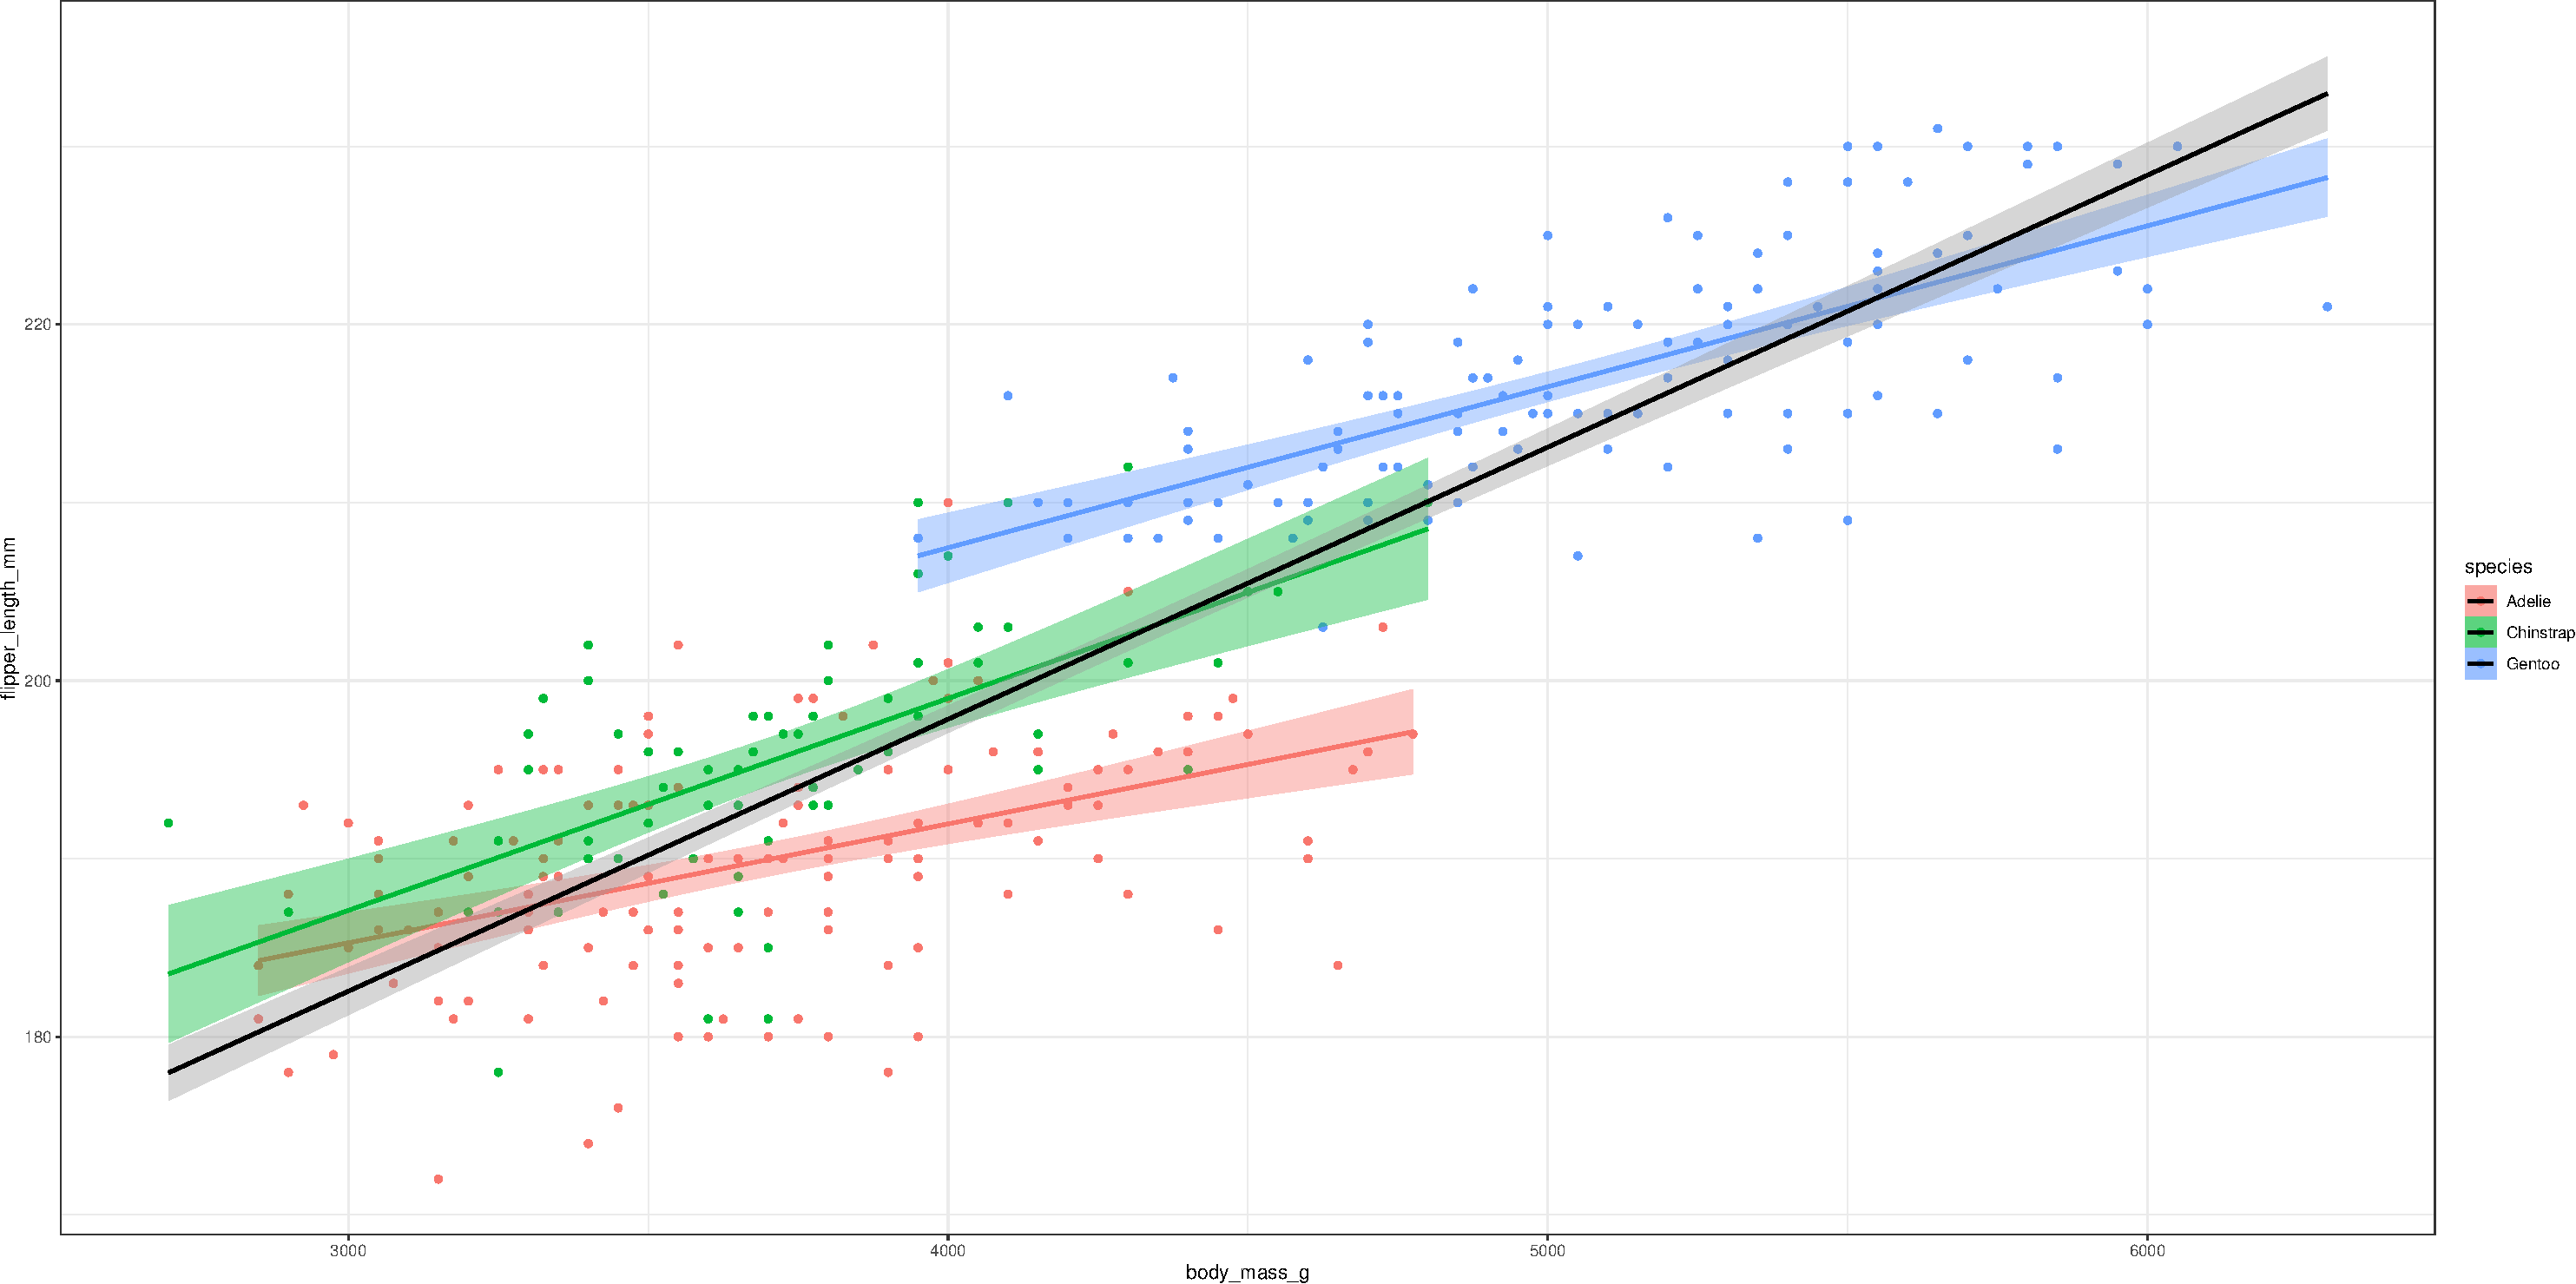
\includegraphics[keepaspectratio]{template_files/figure-pdf/unnamed-chunk-1-1.pdf}}

\end{block}

\end{column}

\separatorcolumn

\begin{column}{\colwidth}

\begin{exampleblock}{A highlighted block containing some math}

A different kind of highlighted block.

\[
\int_{-\infty}^{\infty} e^{-x^2}\,dx = \sqrt{\pi}
\]

Interdum et malesuada fames \(\{1, 4, 9, \ldots\}\) ac ante ipsum primis
in faucibus.

\heading{A heading inside a block}

Praesent consectetur mi \(x^2 + y^2\) metus, nec vestibulum justo
viverra nec.

\end{exampleblock}

\begin{block}{Nullam vel erat at velit convallis laoreet}

Class aptent taciti sociosqu ad litora torquent per conubia nostra, per
inceptos himenaeos.

\end{block}

\end{column}

\separatorcolumn

\begin{column}{\colwidth}

\begin{block}{Results}

Aliquam sit amet urna quis tellus scelerisque congue diam.

\begin{longtable}[]{@{}lrrc@{}}
\caption{A table caption.}\tabularnewline
\toprule\noalign{}
First column & Second & Third & Fourth \\
\midrule\noalign{}
\endfirsthead
\toprule\noalign{}
First column & Second & Third & Fourth \\
\midrule\noalign{}
\endhead
\bottomrule\noalign{}
\endlastfoot
Foo & 13.37 & 384,394 & \(\alpha\) \\
Bar & 2.17 & 1,392 & \(\beta\) \\
Baz & 3.14 & 83,742 & \(\delta\) \\
\end{longtable}

Donec quis posuere ligula. Nunc feugiat elit a mi malesuada consequat.

\end{block}

\begin{block}{Conclusion}

Proin auctor ante in augue tincidunt tempor. Aenean at velit vel dolor
blandit molestie.

\end{block}

\end{column}

		\separatorcolumn
	\end{columns}
\end{frame}

\end{document}
